\documentclass[a4paper,11pt]{scrartcl}
\usepackage[T1]{fontenc}
\usepackage[utf8]{inputenc}
%\usepackage{lmodern}
\usepackage[top=1.1in, bottom=1.1in, left=1in, right=1in]{geometry}
\usepackage[czech]{babel}
\usepackage{hyperref}
\usepackage{graphicx}
\usepackage{caption}
\usepackage{subcaption}

\addto\captionsczech{\renewcommand{\refname}{}}

\usepackage{minted}
\newminted{ocaml}{fontsize=\small}
\newminted{cpp}{fontsize=\small, fontfamily=tt, mathescape}
\newminted{bash}{fontsize=\small}

\title{Návrh konvolučního filtru pomocí evolučních algoritmů}
\subtitle{Projekt MAPV}
\author{Vojtěch Vladyka a Martin Sehnoutka}

\newcommand{\keyword}{\textbf }

\begin{document}

\maketitle
\tableofcontents

\section{Zadání}
Cílem projektu je navrhnout algoritmus pro indukci konvoluční masky na základě dvou šedotónových nebo barevných obrázků. Pro hledání řešení jsou použité genetické algoritmy. Jako prostředek realizace je zvolena knihovna OpenCV a programovací jazyk C++.

\begin{verbatim}
 +----------+                      +----------+
 | Původní  |                      | Nový     |
 | obrázek  |----> Konvoluce ----> | obrázek  |
 +----------+                      +----------+
\end{verbatim}

\section{Teoretický rozbor}

Práci je možné rozdělit do dvou základních oblastí. První jsou genetické algoritmy, které byly použity pro hledání optimálního řešení. Druhá oblast je zpracování obrazu, jelikož se zabýváme porovnáváním dvou obrázků, námi vytvořeného a zadaného.

Tato sekce je pouhým náznakem principu daných algoritmů, jelikož předpokládáme, že toto není hlavním cílem projektu.

\subsection{Genetické algoritmy}

Jde o heuristický postup, který se snaží aplikovat evoluční principy na optimalizační úlohu. Na rozdíl od analytického výpočtu nepředpokládáme na výstupu exaktní řešení, proto tyto metody používáme v případě, že neznáme analytický postup jak úlohu vyřešit. Celý algoritmus se dá rozdělit na několik kroků, kterým říkáme genetické operátory. Jsou to selekce, křížení a mutace. Tyto operátory potom pracují nad množinou jedinců, kterou nazýváme populace. Jako poslední termín zavádíme fitness funkci, jenž slouží k ohodnocení "výkonnosti" jedince.

\begin{verbatim}
Schéma genetického algoritmu:

  1. Vytvoření počáteční populace
  2. Ohodnocení fitness funkcí
  3. Ukončovací podmínka
      +--> Splněna: Skok na konec 
      +--> Nesplněna: Pokračuj
  4. Selekce
  5. Křížení
  6. Mutace
  7. Elitismus - nejlepšího jedince ponech bez změny
  8. Skok na fitness
\end{verbatim}

\subsection{Selekce}
Naivní řešení by bylo vzít nejlepší jedince ze současné generace a stvořit generaci novou. Tímto postupem bychom se ovšem brzy dostali do lokálního minima, což není žádoucí. Proto zavádíme různé metody selekce, které mají tomuto jevu předcházet tak, že preferují lepší jedince, ale na bázi určité náhody dávají šanci i jedincům horším. V našem projektu implementujeme tyto metody selekce:

\paragraph{Vážená ruleta}
Tato metoda náhodně vybírá jednoho jedince z populace, nicméně lepší jedinci mají vyšší pravděpodobnost. Tato pravděpodobnost je určena poměrem jejich fitness funkcí.

\paragraph{Poziční selekce}
Funguje stejně jako vážená ruleta pouze místo fitness funkce používá pro určení poměrů pravděpodobnosti pozici jedince v pořadí od nejlepšího po nejhoršího. Tato metoda na rozdíl od rulety dává šanci jedincům i v případech, že jejich fitness je podstatně menší než nejlepších jedinců. Tím lze opět eliminovat možnost konvergence do lokálních minim.

\paragraph{Turnaj}
Metoda náhodně vybírá dvojice, ze které vybírá toho lepšího jedince.

\subsection{Křížení}

\paragraph{blx a, simple, convex}

\paragraph{BLX-$\alpha$}
Metoda křížení BLX-$\alpha$ \ref{blx} je založená na principu výběru hodnoty z rozsahu většího, než je rozsah rodičů, takže se může potomek vyhnout lokálnímu extrému.\\
Výsledná hodnota jednoho prvku po křížení je určena takto:
\begin{equation}
    u = <min(x,y) - \alpha \Delta; max(x,y) + \alpha \Delta>
\end{equation}
kde $\alpha$ je parametr rozšíření intervalu, $\Delta$ je absolutní hodnota rozdílu hodnot rodičů. Hodnota $u$ je hodnota nového potomka která je náhodně vybraná z intervalu.

\subsection{Mutace}

\subsection{Zpracování obrazu}

\paragraph{Chybová funkce}

Slouží k ohodnocení podobnosti dvou obrazů, tzn. v našem případě je použita jako fitness funkce pro genetický algoritmus.

\paragraph{Kvadrát rozdílu obrazových funkcí}

Jedná se o naivní implementaci porovnání dvou obrazů, která se dá popsat tímto vzorcem:
\begin{equation}
  error = \sqrt{\sum\limits_{\forall r} \sum\limits_{\forall c} ( O_{r,c} - Y_{r,c} )^2}
\end{equation}

Kde $O$ je vzor upravený neznámým konvolučním jádrem a $Y = I \ast k $ je vzor po konvoluci s kandidátním řešením. $r,c$ jsou obrazové souřadnice.

Tato funkce ovšem vykazuje opačné chování, než jsme od fitness funkce chtěli, klesá s lepším kandidátem a roste s horším. Proto jsme vzorec upravili, aby vyhovoval našim potřebám.
\begin{equation}
  fitness = \sqrt{\frac{rows \cdot cols}{{\sum\limits_{\forall r} \sum\limits_{\forall c} ( O_{r,c} - Y_{r,c} )^2}}}
\end{equation}

Nicméně ani tato fitness funkce nebyla vyhovující neboť dostatečně nerozlišovala dobré a špatné kandidáty, proto jsme ji upravili do finální podoby:
\begin{equation}
  fitness_{new} = e ^ {5 \cdot fitness}
\end{equation}

Kde hodnota 5 byla určena experimentálně.

\paragraph{SSIM}
SSIM (Structural Similiarity Image Assesment) je metoda spadající pod Image Quality Assesment (IQA), která vyjadřuje podobnost dvou obrazů na škále od -1 pro naprosto odlišné obrazy po 1 pro identické obrazy. Tato medota bere vychází ze způsobu jak obraz vnímá člověk, a to že sleduje strukturu obrazu.\\
Definice podle původní práce\cite{ssim} je následující:
\begin{equation}
    SSIM(x,y) = \frac{(2 \mu_x \mu_y + C_1)(2 \sigma_{xy} + C_2)}{({\mu_x}^2 + {\mu_y}^2 + C_1)({\sigma_x}^2 + {\sigma_y}^2 + C_2)}
\end{equation}
kde $\mu$ je průměr hodnot pixelů obrazu, $\sigma$ je standartní odchylka obrazu. Konstanty $C_1$ a $C_2$ jsou odvozeny od rozsahu hodnot pixelu $L$, v našem případě 255 a konstanty $k << 1$. V práci jsou použity hodnoty $k_1 = 0,01$ a $k_2 = 0,03$. Posléze se konstanta $C$ počítá takto: $C = k \cdot L$.\\
V naší implementaci, která byla převzaná ze zdroje \cite{ssim-src} jsou použity konstanty $C_1 = 6,5025$ a $C_2 = 58,5225$. Průměr $\mu$ je řešen pomocí gaussiánu 11x11. Standartní odchylka $\sigma$ je realizována jako rozdíl gaussiánu a $\mu$. Poté je všechno ve formě matice, tím pádem je potřeba pro skalární výsledek spočítat průměrnou hodnotu matice.\\
Tato metoda vykazuje vyšší výpočetní náročnost ale zároveň i lepší výsledky, obzvláště u nedostatečného množství významných bodů.

\section{Implementace}
Jak již bylo zmíněno, implementace byla provedena v jazyku C++ a to s pomocí knihovny OpenCV. Samozřejmě jsme nepoužili pouze tuto knihovnu, ale rovněž STL, Google test framework, boost atd. I přes použitý jazyk, jsme implementaci neprovedli čistě objektově. Většina základních funkcí (jako jsou na příklad genetické operátory) jsou definovány jako prosté funkce, u kterých byl důraz kladen na ortogonalitu a modularitu, abychom mohli jednoduše zkoušet různé kombinace námi implementovaných operátorů. Nicméně pro pohodlné použití jsme vytvořili jednu třídu příhodně nazvanou Worker, která zapouzdřuje celý genetický algoritmus, ta obsahuje parametry generace a ukazatele na použité operátory.


Testování programu je možné pomocí dvou spustitelných souborů. První z nich je \uv{gekon\_run}, který jako parametry přebírá velikost konvolučního jádra a vstupní obrázky, nicméně nelze měnit parametry algoritmu neboť jsou, jak by se řeklo v IT žargonu, \uv{hardcoded} ve zdrojovém souboru. Tento problém řeší druhý spustitelný soubor, který je pojmenován \uv{automated\_tests} a přebírá konfigurační soubor napsaný v jazyku TOML, ten pak definuje parametry testů jako jsou např. velikost generace, použité operátory a počet vláken.


Struktura projektu:
\begin{verbatim}
. -- bin -- spustitelné soubory
  |- docs -- dokumentace
  |- gekon -- zdrojové kódy
  |- samples -- testovací vzory
  |- tests -- unit testy
\end{verbatim}

Ukázka rozhraní genetických operátorů:
\begin{cppcode}
typedef std::function<std::vector<candidate_t>(candidate_t, candidate_t)> crossover_fcn_t;
typedef std::function<void(candidate_t&, unsigned int, unsigned int)> mutation_fcn_t;
typedef std::function<double(tr_sample_t, candidate_t)> fitness_fcn_t;
typedef std::function<population_t(population_t)> selection_fcn_t;
\end{cppcode}

A implementace jednoho konkrétního operátoru:
\begin{cppcode}
void m_dynamic(candidate_t &X, unsigned int t, unsigned int T) {
    /*
     * Dynamic mutation (Michalewicz):
     * Defined as $\Delta(t,y) = y \left( 1 - r^{ {1-\frac{t}{T} }^B }  \right)$
     *     where B = 5
     */
    int rows = X.rows;
   	int cols = X.cols;
   	for (int r = 0; r < rows; ++r) {
        for (int c = 0; c < cols; ++c) {
            if(random(0,1) < m_swap_prob) {
                X.at<ker_num_t>(r,c) = X.at<ker_num_t>(r,c)*
                (1-pow(random(0,1), pow(float(1)-float(t)/T, m_dynamic_B)));
            }
        }
    }
}

\end{cppcode}

\subsection{Spouštění testů}
Program během výpočtů vypisuje průběžné výsledky. Ideální je výstup (stdout) přesměrovat do souboru a následně filtrovat požadované informace. Jako příklad uvádíme srovnání časové náročnosti běhu jednotlivých algoritmů:
\begin{bashcode}
$ cat example1.log | grep '\[TEST\]' | grep  'Time elapsed\|Test name'
[TEST]Test name: tournament-blx_a-ssim-swap
[TEST]Time elapsed: 1021
[TEST]Test name: tournament-simple-mse-dynamic
[TEST]Time elapsed: 579
[TEST]Test name: tournament-blx_a-ssim-dynamic
[TEST]Time elapsed: 1050
[TEST]Test name: tournament-blx_a-mse-swap
[TEST]Time elapsed: 597
[TEST]Test name: tournament-simple-mse-swap
[TEST]Time elapsed: 611
[TEST]Test name: tournament-simple-ssim-dynamic
\end{bashcode}

\section{Zhodnocení dosažených výsledků}
Během testování jsme vyzkoušeli všechny možné kombinace námi napsaných operátorů nad všemi zadanými vzory. Časová náročnost byla přibližně jeden den na výkonném domacím počítači při fixní délce běhu 500 iterací. 

\subsection{Vizuální porovnání výsledků}
Při pohledu na výsledky lze usuzovat vhodnost některých metod pro tuto úlohu. Např. fitness funkce kvadrátu odchylky dává stabilně horší výsledky než SSIM, to samé lze tvrdit o mutaci metodou swap oproti dynamické mutaci, jejíž výsledky jsou z pravidla lepší. Naopak vliv selekce a křížení je spíše menší. Ten by se projevil hlavně na rychlosti konvergence k výsledku.

%Obrázek \ref{porovnani} zobrazuje vybrané výsledky našich algoritmů ve srovnání s trénovacím vzorem.

Obrázek \ref{porovnani_ex1} ukazuje výsledky různých kombinací operátorů. Výsledek \ref{fig:ex11} je vizuálně nejshodnější, zatímco výsledek \ref{fig:ex12} se v jistých bodech odlišuje více (byť to není v těchto malých náhledech vidět). Naopak výsledek \ref{fig:ex13} je evidentně špatně, ačkoli možná by se po delším čase dostal též k výsledku.

Jak bude vidět na dalších ukázkách, kombinace operátorů Roulette pro selekci, BLX-$\alpha$ pro křížení, SSIM pro fitness a Dynamická mutace se jeví jako nejlepší kombinace univerzálně pro všechny zadané vzory.

Zajíámavá situace je vidět na obrázku \ref{porovnani_ex2}. Správný výsledek je opět na obrázku \ref{fig:ex21}, ale rozdíl mezi ním a obrázkem \ref{fig:ex22} je pouze v použitém operátoru mutace, kde v prvním případě je použit lepší operátor Dynamické mutace zatímco ve druhém případě je operátor Swap. Na obrázku \ref{fig:ex23} je evidentně špatný výsledek, který pouze zvýraznil hrany.

Výsledek na šedotónovém obrázku \ref{porovnani_ex6} je obecně lepší, ale i zde jsou výsledky, které jsou naprosto špatně. Správný výsledek je opět na obrázku \ref{fig:ex61} se stále stejnou kombinací jako všechny předchozí příklady. Zajímavá situace nastala u výsledků \ref{fig:ex62} a \ref{fig:ex63}. První jmenovaný je poměrně obstojný. Nemá na správný výsledek, protože je poněkud tmavší, ale řešení je to správné. Ale od špatného výsledku na druhém zmiňovaném se liší pouze způsobem křížení, kde v prvním případě byla použita metoda Simple crossover a u druhého Convex crossover. V tomto případě by bylo zajímavé nechat testy běžet opakovaně, zda se tento výsledek projeví znovu.

Zajímavá změna je na obrázku \ref{porovnani_ex3}. Zde ve vizuální podobnosti vyšel lépe vzorek využívající selekci Turnaj oproti Ruletě. Opět jako několikrát předtím, špatný výsledek je na \ref{fig:ex33}.


\subsection{Porovnání časové náročnosti}

Následující tabulka uvádí vliv jednotlivých operátorů na celkovou časovou náročnost; tzn. nejedná se o náročnost pouze daného operátoru, ale celého algoritmu s použitím tohoto operátoru.

\begin{table}[!h]
  \caption{Porovnání časové náročnosti}
  \label{tab:por}

  \begin{center}
    \begin{tabular}{|c|c|}
    \hline
       Metoda & Průměrný čas [s] \\
       \hline
       SSIM & 448 \\
        mse &
        246 \\
        Turnaj &
        347 \\
        Poziční selekce &
        346 \\
        Ruleta &
        348 \\
        Jednoduché křížení &
        349 \\
        Konvexní křížení &
        347 \\
        BLX-$\alpha$ &
        345 \\
        Mutace swap &
        346 \\
        Mutace dynamická &
        347 \\
        \hline
    \end{tabular}
  \end{center}
\end{table}

Jak je vidět, vliv na celkový čas mají prakticky pouze metody fitness funkce. U genetických operátorů by bylo třeba měřit pouze čas provádění daného operátoru.

\section{Použitá literatura}
%TODO: Doplnit i další zdroje

\begin{thebibliography}{9}
 
\bibitem{strojove-uceni}
HONZÍK, Petr. \emph{Strojové učení} [online]. Brno, 2006. Dostupné také z: \url{www.vutbr.cz}

\bibitem{ssim}
WANG, Zhou, Alan C. BOVIK, Hamid R. SHEIKH a Eero P. SIMONCELLI. \emph{The SSIM Index for Image Quality Assessment}. The Center for Neural Science at NYU [online]. New York: NY University, 2003 [cit. 2016-04-18]. Dostupné z: \url{http://www.cns.nyu.edu/lcv/ssim/}

\bibitem{blx}
\emph{Blend (BLX) Crossover}. Tomasz Gwiazda e-books [online]. Warsaw: Warsaw University, 2006 [cit. 2016-05-01]. Dostupné z: \url{http://www.tomaszgwiazda.com/blendX.htm}

\end{thebibliography}

\newpage
\section{Přílohy}

%\begin{figure}[!h]
%    \centering
%    \begin{subfigure}[b]{0.4\textwidth}
%        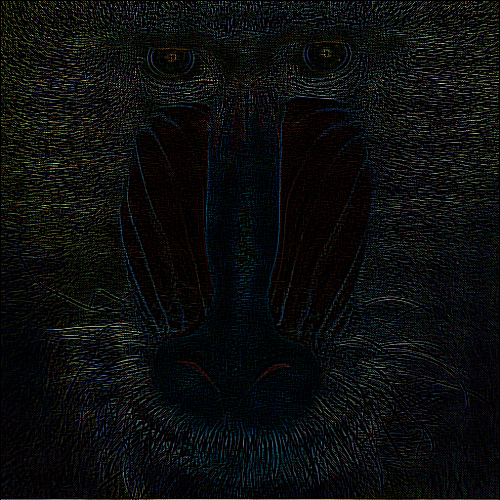
\includegraphics[width=\textwidth]{img/example1_E.png}
%        \caption{První vzor}
%        \label{fig:gull}
%    \end{subfigure}
%    \begin{subfigure}[b]{0.4\textwidth}
%        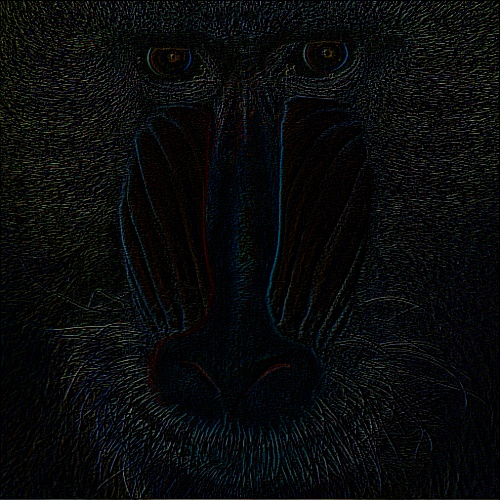
\includegraphics[width=\textwidth]{img/ranksel-simple-ssim-dynamic_example1.jpg}
%        \caption{Povedený pokus (rank selection, simple crossover, ssim, dynamic mutation)}
%        \label{fig:gull}
%    \end{subfigure}
%        \begin{subfigure}[b]{0.4\textwidth}
%        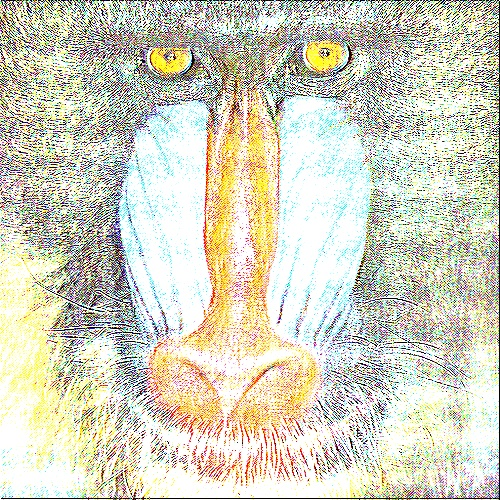
\includegraphics[width=\textwidth]{img/ranksel-convex-mse-swap_example1.jpg}
%        \caption{Nepovedený pokus (rank selection, convex crossover, mse, swap mutation)}
%        \label{fig:gull}
%    \end{subfigure}
%        \begin{subfigure}[b]{0.4\textwidth}
%        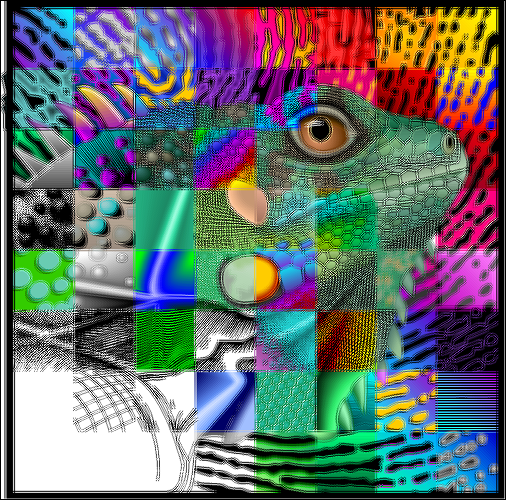
\includegraphics[width=\textwidth]{img/example2_E.png}
%        \caption{Druhý vzor}
%        \label{fig:gull}
%    \end{subfigure}
%        \begin{subfigure}[b]{0.4\textwidth}
%        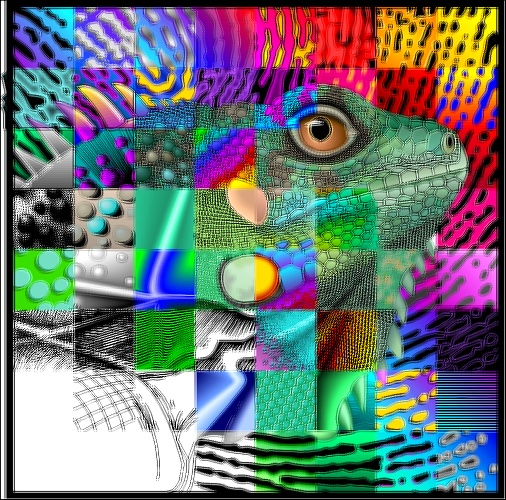
\includegraphics[width=\textwidth]{img/roulette-blx_a-ssim-dynamic_example2.jpg}
%        \caption{Povedený pokus (roulette selection, blx\_a crossover, ssim, dynamic mutation)}
%        \label{fig:gull}
%    \end{subfigure}
%        \begin{subfigure}[b]{0.4\textwidth}
%        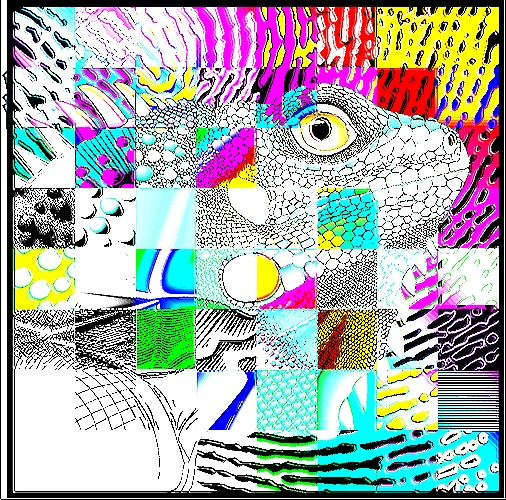
\includegraphics[width=\textwidth]{img/tournament-convex-mse-swap_example2.jpg}
%        \caption{Nepovedený pokus (tournament selection, convex crossover, mse, swap mutation)}
%        \label{fig:gull}
%    \end{subfigure}
%    \caption{Porovnání výsledků}
%    \label{porovnani}
%\end{figure}

\begin{figure}[!h]
    \centering
    \begin{subfigure}[b]{0.32\textwidth}
        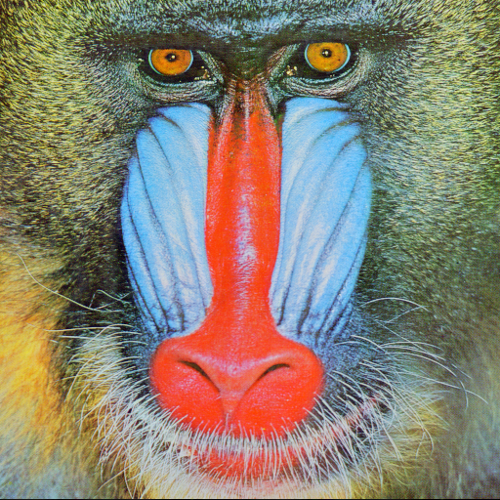
\includegraphics[width=\textwidth]{img/example1.png}
        \caption{Vzor}
        \label{fig:gull}
    \end{subfigure}
    \begin{subfigure}[b]{0.32\textwidth}
        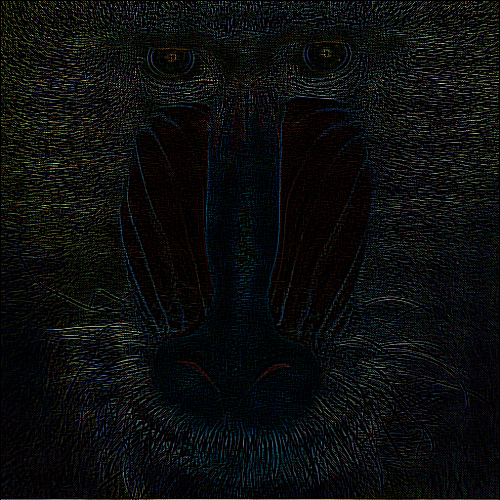
\includegraphics[width=\textwidth]{img/example1_E.png}
        \caption{Požadovaný výsledek}
        \label{fig:gull}
    \end{subfigure}
    \\
    \begin{subfigure}[b]{0.32\textwidth}
        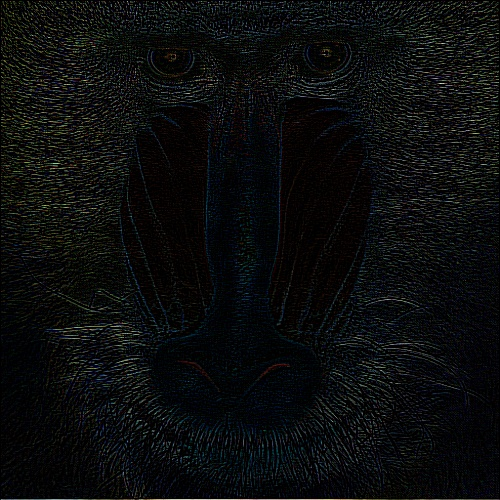
\includegraphics[width=\textwidth]{img/roulette-blx_a-ssim-dynamic_example1.jpg}
        \caption{Správný výsledek (Roulette, BLX-$\alpha$, SSIM, Dynamic mutation)}
        \label{fig:ex11}
    \end{subfigure}
    \begin{subfigure}[b]{0.32\textwidth}
        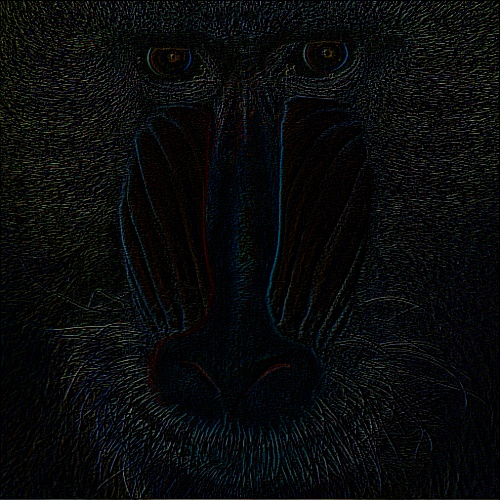
\includegraphics[width=\textwidth]{img/ranksel-simple-ssim-dynamic_example1.jpg}
        \caption{Obstojný výsledek (Rank selection, Simple crossover, SSIM, Dynamic mutation)}
        \label{fig:ex12}
    \end{subfigure}
    \begin{subfigure}[b]{0.32\textwidth}
        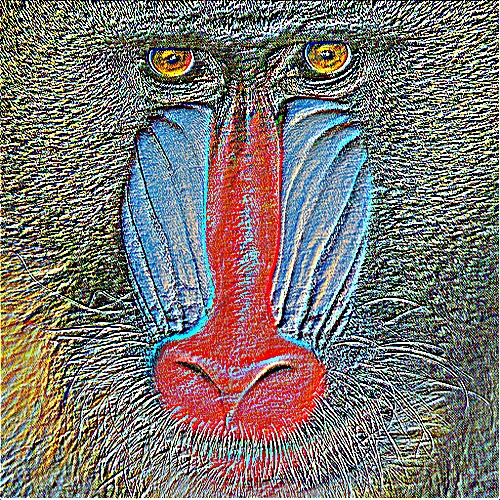
\includegraphics[width=\textwidth]{img/ranksel-blx_a-mse-swap_example1.jpg}
        \caption{Špatný výsledek (Rank selection, BLX-$\alpha$, MSE, Swap mutation)}
        \label{fig:ex13}
    \end{subfigure}
    \caption{Srovnání na vzoru 1}
    \label{porovnani_ex1}
\end{figure}

\begin{figure}[!h]
    \centering
    \begin{subfigure}[b]{0.32\textwidth}
        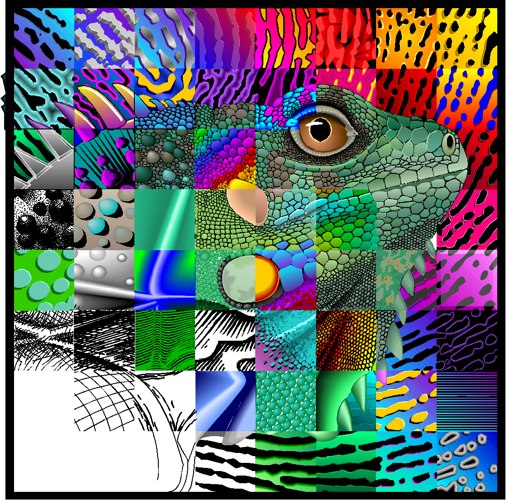
\includegraphics[width=\textwidth]{img/example2.png}
        \caption{Vzor}
        \label{fig:gull}
    \end{subfigure}
    \begin{subfigure}[b]{0.32\textwidth}
        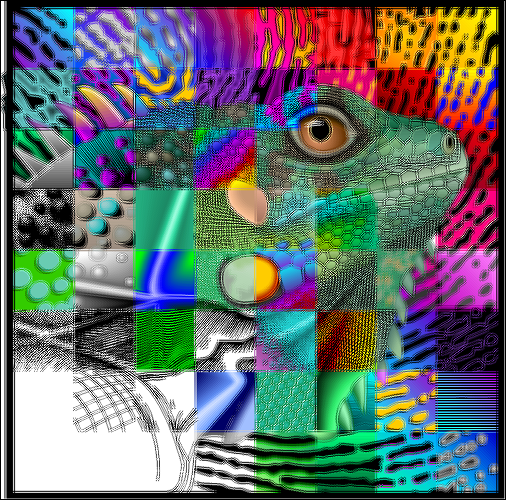
\includegraphics[width=\textwidth]{img/example2_E.png}
        \caption{Požadovaný výsledek}
        \label{fig:gull}
    \end{subfigure}
    \\
    \begin{subfigure}[b]{0.32\textwidth}
        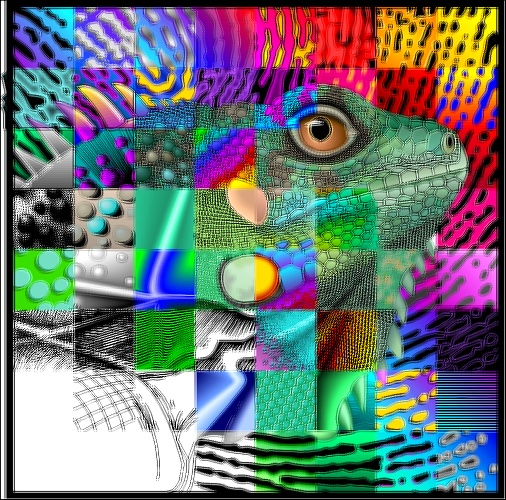
\includegraphics[width=\textwidth]{img/roulette-blx_a-ssim-dynamic_example2.jpg}
        \caption{Správný výsledek (Roulette, BLX-$\alpha$, SSIM, Dynamic mutation)}
        \label{fig:ex21}
    \end{subfigure}
    \begin{subfigure}[b]{0.32\textwidth}
        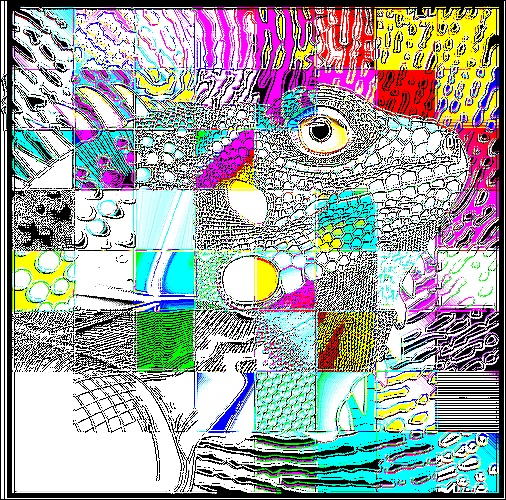
\includegraphics[width=\textwidth]{img/roulette-blx_a-ssim-swap_example2.jpg}
        \caption{Špatný výsledek (Roulette, BLX-$\alpha$, SSIM, Swap mutation)}
        \label{fig:ex22}
    \end{subfigure}
    \begin{subfigure}[b]{0.32\textwidth}
        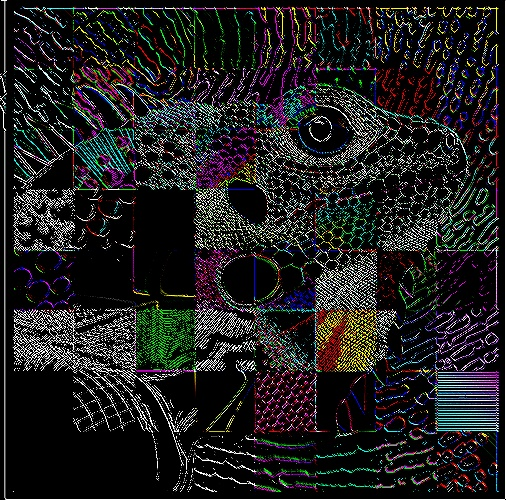
\includegraphics[width=\textwidth]{img/ranksel-convex-mse-swap_example2.jpg}
        \caption{Špatný výsledek (Rank selection, Convex, MSE, Swap mutation)}
        \label{fig:ex23}
    \end{subfigure}
    \caption{Srovnání na vzoru 2}
    \label{porovnani_ex2}
\end{figure}

\begin{figure}[!h]
    \centering
    \begin{subfigure}[b]{0.32\textwidth}
        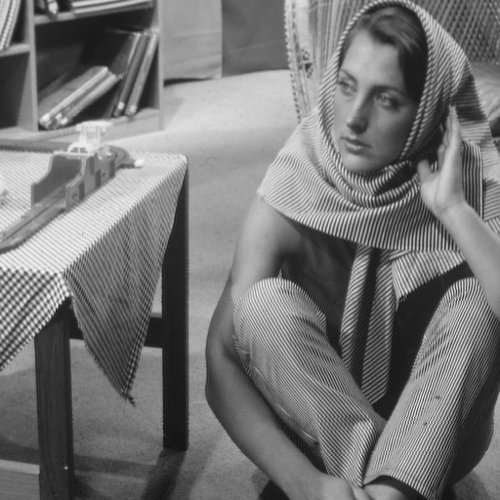
\includegraphics[width=\textwidth]{img/example6.png}
        \caption{Vzor}
        \label{fig:gull}
    \end{subfigure}
    \begin{subfigure}[b]{0.32\textwidth}
        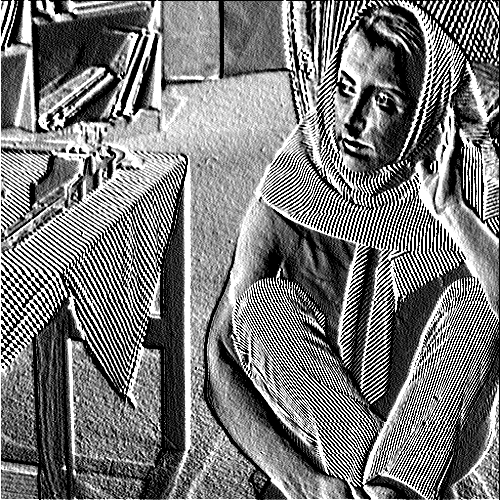
\includegraphics[width=\textwidth]{img/example6_E.png}
        \caption{Požadovaný výsledek}
        \label{fig:gull}
    \end{subfigure}
    \\
    \begin{subfigure}[b]{0.32\textwidth}
        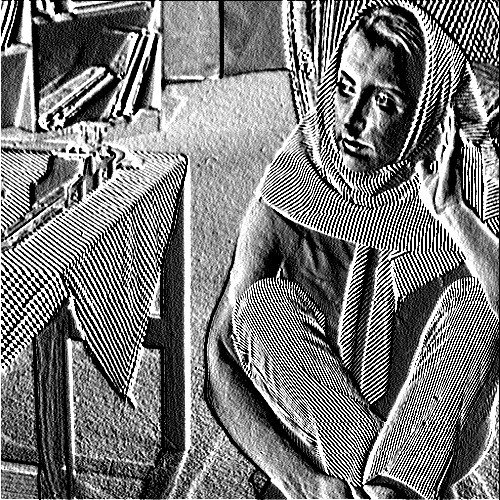
\includegraphics[width=\textwidth]{img/roulette-blx_a-ssim-dynamic_example6.jpg}
        \caption{Správný výsledek (Roulette, BLX-$\alpha$, SSIM, Dynamic mutation)}
        \label{fig:ex61}
    \end{subfigure}
    \begin{subfigure}[b]{0.32\textwidth}
        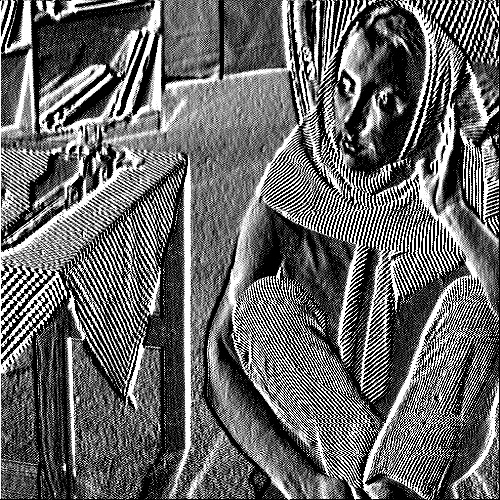
\includegraphics[width=\textwidth]{img/ranksel-simple-mse-swap_example6.jpg}
        \caption{Obstojný výsledek (Rank selection, Simple, MSE, Swap mutation)}
        \label{fig:ex62}
    \end{subfigure}
    \begin{subfigure}[b]{0.32\textwidth}
        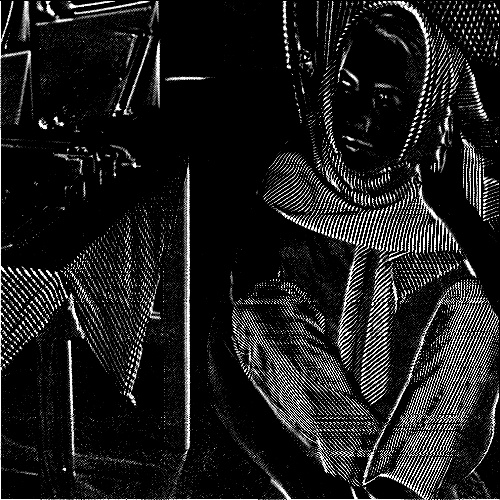
\includegraphics[width=\textwidth]{img/ranksel-convex-mse-swap_example6.jpg}
        \caption{Špatný výsledek (Rank selection, Convex, MSE, Swap mutation)}
        \label{fig:ex63}
    \end{subfigure}
    \caption{Srovnání na vzoru 6}
    \label{porovnani_ex6}
\end{figure}

\begin{figure}[!h]
    \centering
    \begin{subfigure}[b]{0.32\textwidth}
        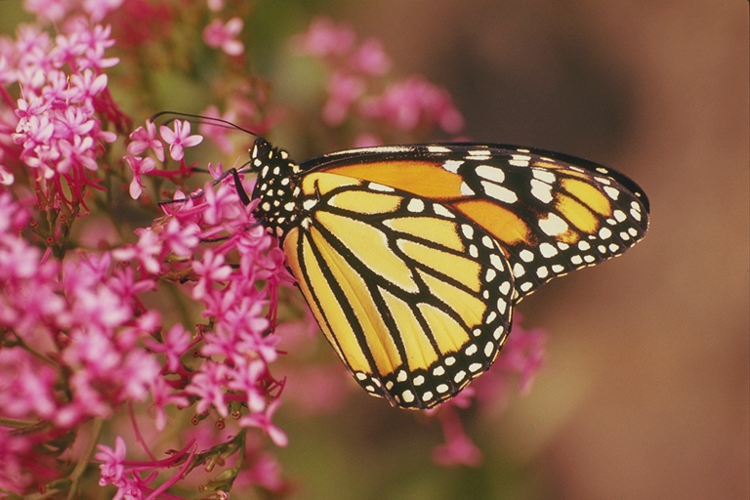
\includegraphics[width=\textwidth]{img/example3.png}
        \caption{Vzor}
        \label{fig:gull}
    \end{subfigure}
    \begin{subfigure}[b]{0.32\textwidth}
        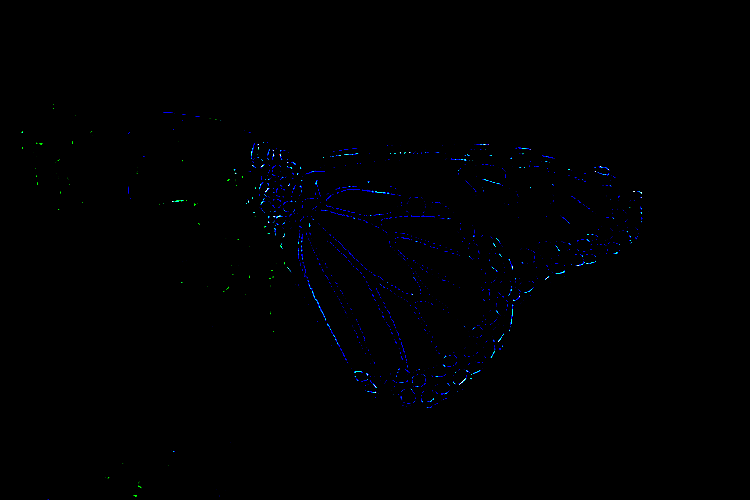
\includegraphics[width=\textwidth]{img/example3_E.png}
        \caption{Požadovaný výsledek}
        \label{fig:gull}
    \end{subfigure}
    \\
    \begin{subfigure}[b]{0.32\textwidth}
        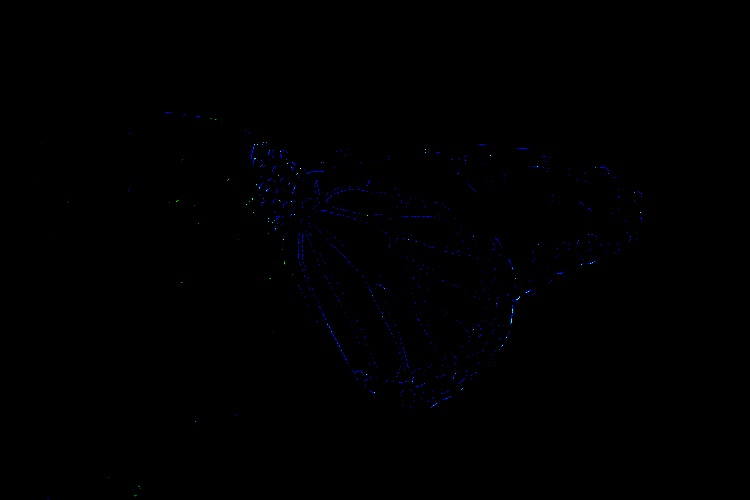
\includegraphics[width=\textwidth]{img/tournament-blx_a-ssim-dynamic_example3.jpg}
        \caption{Správný výsledek (Tournament (!), BLX-$\alpha$, SSIM, Dynamic mutation)}
        \label{fig:ex31}
    \end{subfigure}
    \begin{subfigure}[b]{0.32\textwidth}
        
\includegraphics[width=\textwidth]{img/roulette-blx_a-ssim-dynamic_example3.jpg}
        \caption{Správný výsledek (Roulette, BLX-$\alpha$, SSIM, Dynamic mutation)}
        \label{fig:ex32}
    \end{subfigure}
    \begin{subfigure}[b]{0.32\textwidth}
        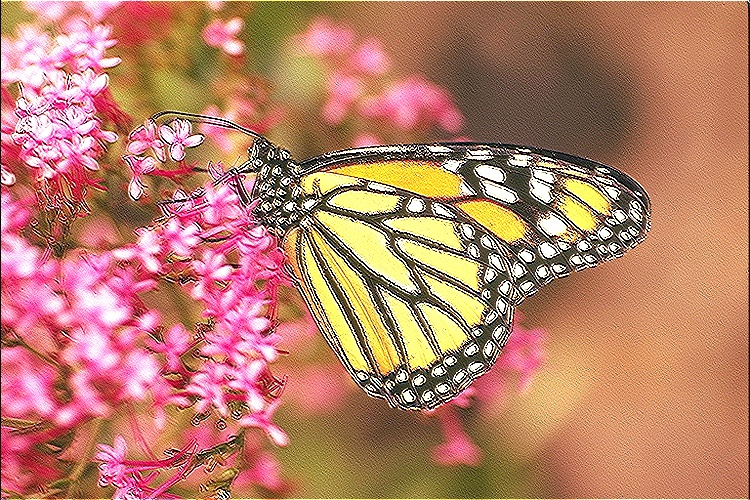
\includegraphics[width=\textwidth]{img/roulette-convex-mse-swap_example3.jpg}
        \caption{Špatný výsledek (Roulette, Convex, MSE, Swap mutation)}
        \label{fig:ex33}
    \end{subfigure}
    \caption{Srovnání na vzoru 3}
    \label{porovnani_ex3}
\end{figure}

\begin{figure}[!h]
    \centering
    \begin{subfigure}[b]{0.4\textwidth}
        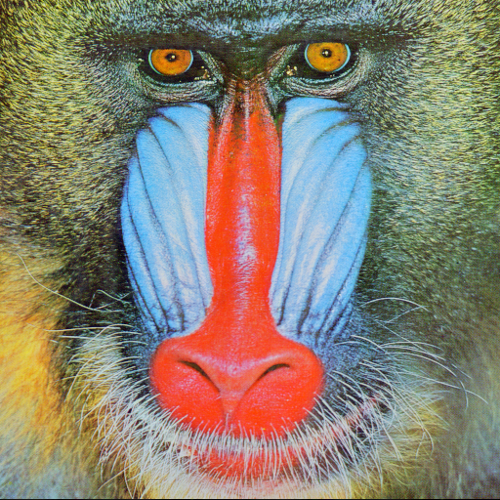
\includegraphics[width=\textwidth]{img/example1.png}
        \caption{Vzor 1}
        \label{fig:gull}
    \end{subfigure}
    \begin{subfigure}[b]{0.4\textwidth}
        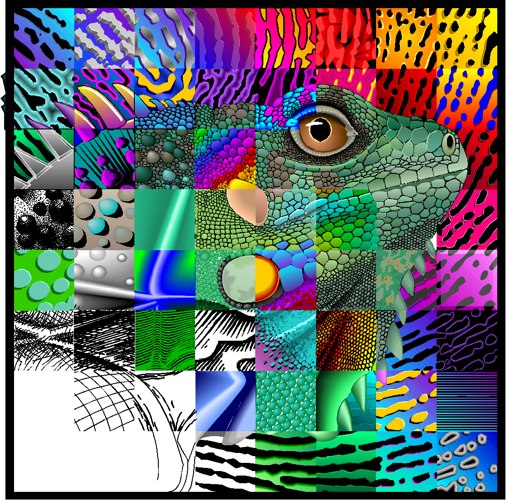
\includegraphics[width=\textwidth]{img/example2.png}
        \caption{Vzor 2}
        \label{fig:gull}
    \end{subfigure}
    \begin{subfigure}[b]{0.4\textwidth}
        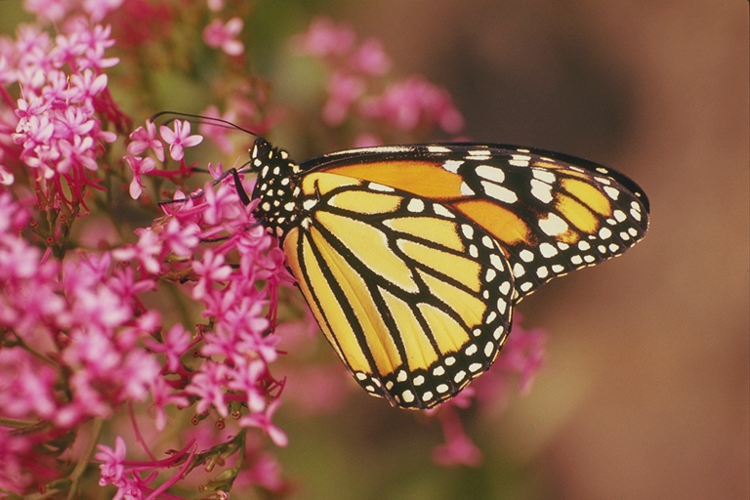
\includegraphics[width=\textwidth]{img/example3.png}
        \caption{Vzor 3}
        \label{fig:gull}
    \end{subfigure}
    \begin{subfigure}[b]{0.4\textwidth}
        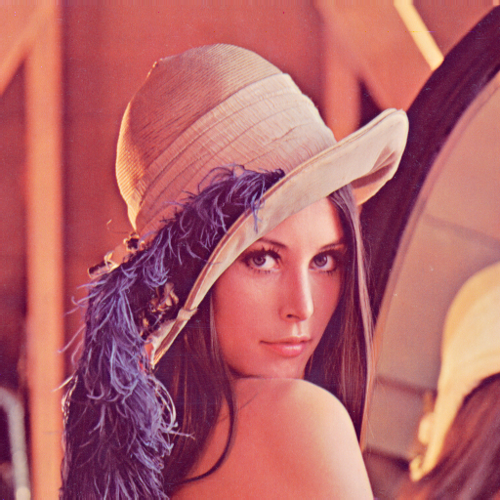
\includegraphics[width=\textwidth]{img/example4.png}
        \caption{Vzor 4}
        \label{fig:gull}
    \end{subfigure}
    \begin{subfigure}[b]{0.4\textwidth}
        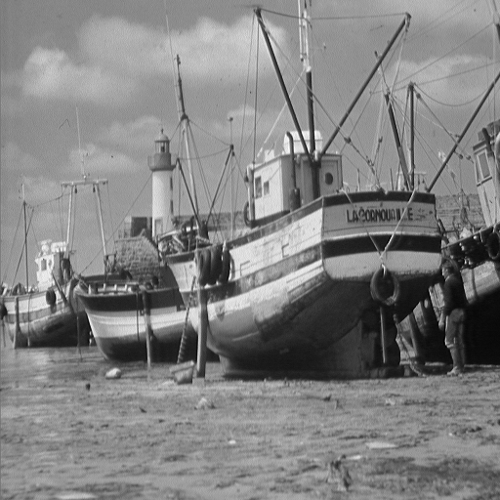
\includegraphics[width=\textwidth]{img/example5.png}
        \caption{Vzor 5}
        \label{fig:gull}
    \end{subfigure}
    \begin{subfigure}[b]{0.4\textwidth}
        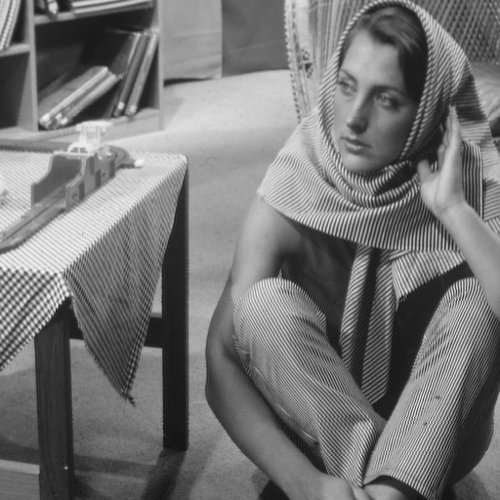
\includegraphics[width=\textwidth]{img/example6.png}
        \caption{Vzor 6}
        \label{fig:gull}
    \end{subfigure}
    \caption{Vzory}
    \label{vzory}    
\end{figure}


\end{document}
